\chapter{MODELO DE VELOCIDADES DE BACKGROUND}
\label{cap3}

A primeira iteração do algoritmo de inversão tem por objetivo a obtenção do gradiente de
velocidades em profundidade do modelo de velocidades de background \cite{niptomo,stereo}.
O modelo inicial utilizado é um modelo de velocidades homogêneo
e de velocidade constante igual a $1.5Km/s$,
correspondente a velocidade próxima da superfície de aquisição. Traçamos raios normais
partindo da coordenada $m_0$ e com ângulo de inclinação $\beta_0$ em direção ao modelo
de velocidade constante para determinar a localização inicial das fontes PIN (cruzes
em preto na Figura \ref{fig:3.1}). Este será o modelo inicial desta etapa da inversão.

\begin{figure}[H]
\caption{Modelo de velocidade constante utilizado para a configuração inicial da
posição das fontes pontuais PIN (cruzes em preto).}
\begin{center}
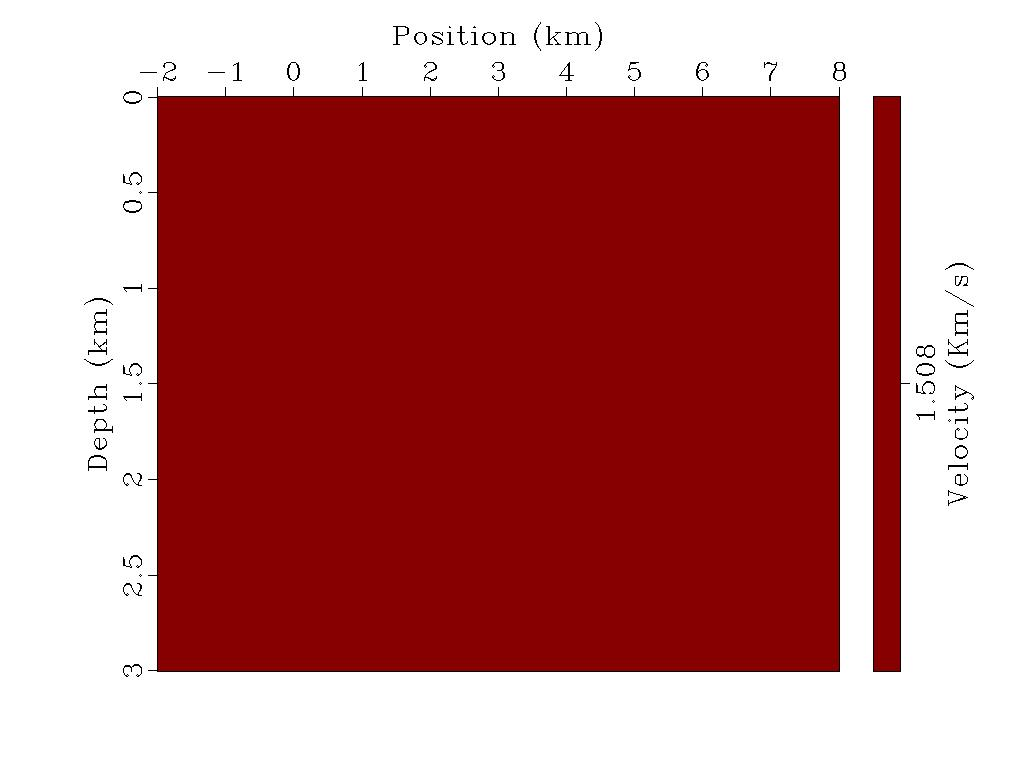
\includegraphics[scale=0.3]{images/ctevel.jpeg}
\vspace{-0.3cm}
\end{center}
\begin{center}
 Fonte: Do Autor.
\end{center}
\label{fig:3.1}
\end{figure}


Para a otimização do modelo de velocidades de gradiente constante
é utilizada a Equação \ref{eq:2.2} da soma das
diferenças nos tempos de trânsito obtidos com o tratamento de raios e os tempos de trânsito calculados utilizando a fórmula do ERC (Equação \ref{eq:2.1}). Utilizamos o algoritmo Very Fast Simulated Annealing (VFSA) para atualizar o gradiente em profundidade do modelo de velocidades.
O modelo de velocidades é atualizado a cada iteração do algoritmo para cada valor do gradiente e segue a seguinte função de velocidades:

\begin{equation}
\label{eq:4.1}
v(z)=z g_z+v_0
\end{equation}

Em \ref{eq:4.1} a velocidade $v(z)$ cresce linearmente com a profundidade.

O valor mínimo da diferença entre os tempos de trânsito (Equação \ref{eq:2.2})
será obtido para o gradiente de velocidades ótimo.
O valor do gradiente é armazenado e utilizado para gerar o modelo de velocidades
da Figura \ref{fig:3.2}. Este modelo será o modelo de background utilizado na etapa seguinte
da inversão do modelo de velocidades com variação lateral de velocidade.

O gradiente de velocidades obtido é $g_z=0.1673 s^-1$. O modelo de velocidades resultante é apresentado na
Figura \ref{fig:3.2} à direita em comparação com o modelo de velocidade constante na Figura \ref{fig:3.2}
à esquerda, as cruzes em preto representam a localização das fontes pontuais PIN em cada um dos modelos.
A localização das fontes pontuais PIN obtidas a partir do modelo de velocidades de gradiente constante
é plotada sobre o modelo de velocidades original na Figura \ref{fig:3.3}.

\begin{figure}[H]
\caption{Modelo de velocidade constante à esquerda (velocidade igual a $1.5Km/s$)
e o modelo de velocidades com gradiente constante à direita
(o gradiente de velocidades em profundidade é $0.1673 s^-1$).
As cruzes em preto representam a localização das fontes PIN.}
\begin{center}
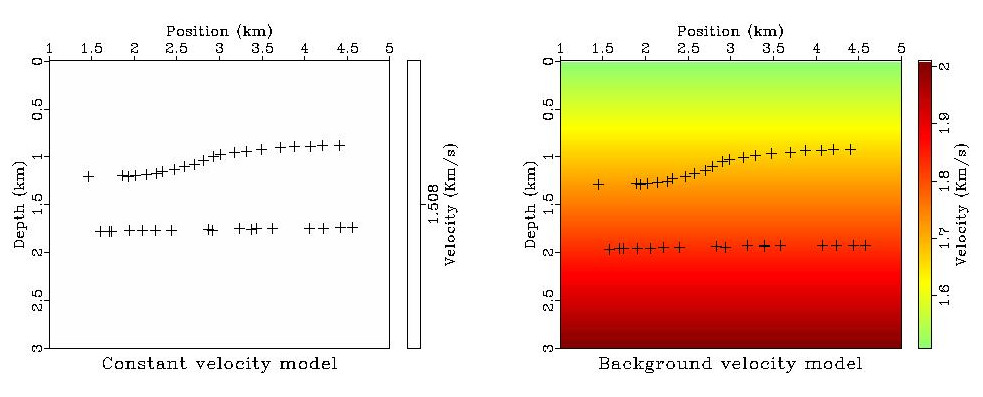
\includegraphics[scale=2]{images/compare.jpeg}
\vspace{-0.3cm}
\end{center}
\begin{center}
 Fonte: Do Autor.
\end{center}
\label{fig:3.2}
\end{figure}

\begin{figure}[H]
\caption{Localização das fontes pontuais PIN (cruzes em preto)
obtidas com o modelo de velocidades de gradiente
constante plotada sobre o modelo de velocidades original.
Compare a localização das cruzes com a posição dos refletores.}
\begin{center}
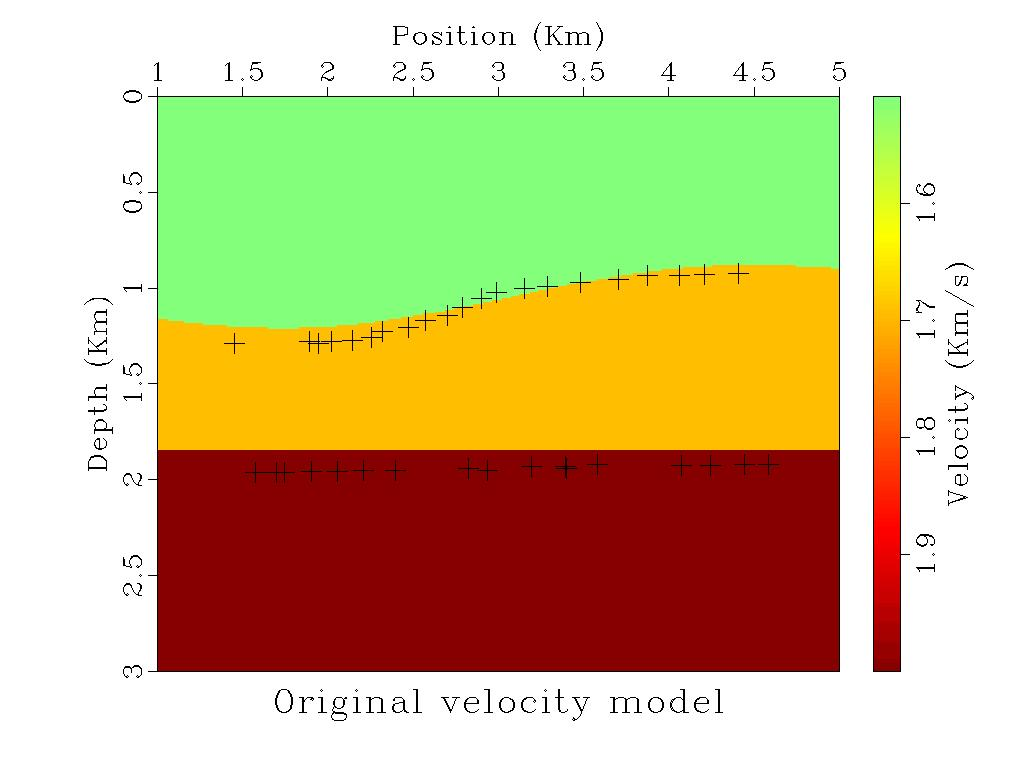
\includegraphics[scale=0.3]{images/gzvel.jpeg}
\vspace{-0.3cm}
\end{center}
\begin{center}
 Fonte: Do Autor.
\end{center}
\label{fig:3.3}
\end{figure}


\begin{figure}[H]
\caption{Localização das fontes PIN obtidas no modelo de velocidade constante
plotadas sobre o modelo de velocidades original (à esquerda)
e localização das fontes PIN obtidas no modelo de velocidades com gradiente constante
plotadas sobre o modelo de velocidades original (à direita).
As cruzes em preto representam a localização das fontes PIN.}
\begin{center}
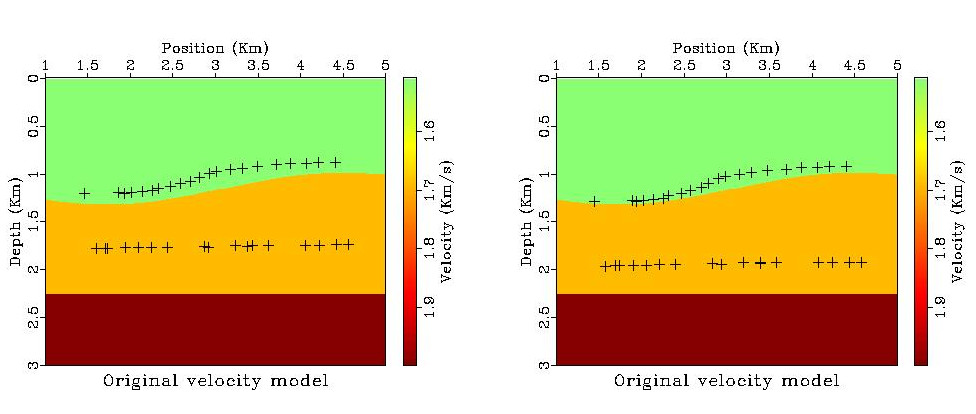
\includegraphics[scale=2]{images/resultinv.jpeg}
\vspace{-0.3cm}
\end{center}
\begin{center}
 Fonte: Do Autor.
\end{center}
\label{fig:3.4}
\end{figure}
